% !TeX root = paper.tex


\chapter{システムについて}\label{system}
%\section{この章で書くこと}
%\begin{itemize}
%	\item 識別,分類とは
%	\item 現存するサービスでできること
%	\item 概要図
%	\item モデルについて
%	\item サーバ関連について
	%\item もしかしたらあんまり書くことないかも
%\end{itemize}
\section{分類と識別とは}
%参考文献:https://business.ntt-east.co.jp/content/cloudsolution/column-391.html
分類はデータやオブジェクトを異なるクラスやカテゴリに分けるプロセスを指す.画像の分類とは,画像が特定のカテゴリやクラスに属するかどうかを判別する作業である.例えば,画像に写っているのが猫か犬かのクラスに分けることである.

識別とは画像のどこに何が写っているのかを判別するプロセスを指す.1枚の画像に複数の物体が存在する場合も識別はできる.動画に写っている電車の車両タイプも判別することができる.



\section{現存するサービス}
現在車両タイプを調べるためには,Googleレンズを利用することや図鑑と見比べることの2つが挙げられる.
Google レンズとは画像の分類を行うアプリである.単に分類結果が表示されるのではなく,分類したいオブジェクトが映っているWebページ一覧が表示されるものである.表示されたWebページを適当に選び自分が知りたい結果をWebページの中から探し出す必要がある.また,一枚の画像に複数のオブジェクトが存在している場合は正しい結果が得られない.


\section{YOLO}
YOLOとはYou Only Look Onceの略で,人間のように一目見るだけで物体検出ができることを指している\cite{YOLO}.データセットを作成し学習させることで,任意の物体のみ検出させることが可能である.
YOLOv8はYOLOシリーズの最新バージョンであり,ディープラーニングとコンピュータビジョンの最先端の進歩に基づいており,速度と精度の麺で比類のない性能を提供している.
%https://docs.ultralytics.com/ja/ 参照
本プロジェクトでは,YOLOv8を用いて電車の車両タイプを識別,分類する2つのモデルを開発する.

\section{システム概要図}
本プロジェクトで開発するシステム概要を図\ref{FIG}に示す.システムは車両判別部とUIに分けられる.

\begin{figure}
	\centering
	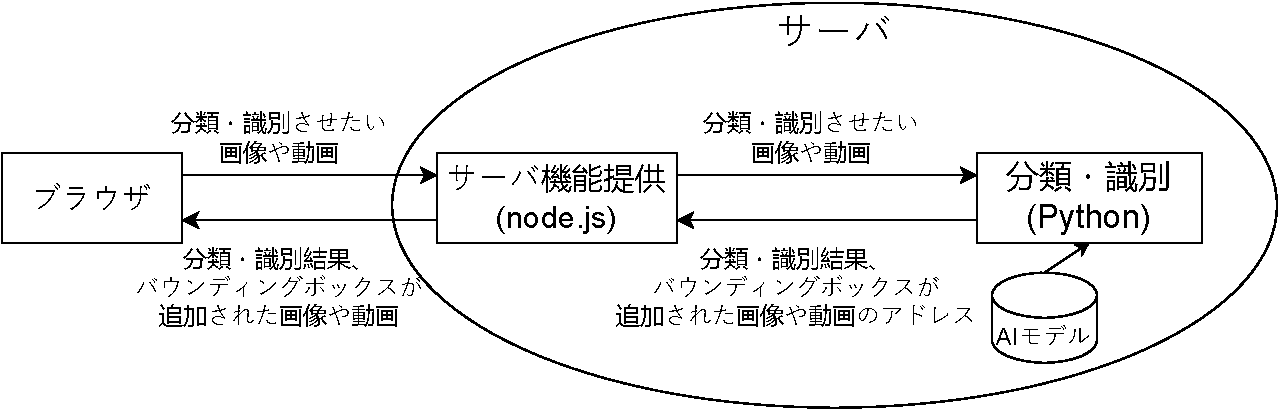
\includegraphics [width=\linewidth]{chap2/fig/sys_gaiyou6.pdf}
	\caption{システム概要図}
	\label{FIG}
\end{figure}

\section{システムの機能}
%本システムの機能として電車の分類と識別を提供する.識別は動画と画像の両方に対応している.
%画像や動画を入力すると,判別結果が出力される.
本システムは,以下の3つの機能を提供する.
%本システムは,電車の画像の分類と電車の画像と動画の識別の3つ機能を提供する
\begin{itemize}
	\item 電車の画像の分類
	\item 電車の画像の識別
	\item 電車の動画の識別
\end{itemize}





\section{動作環境}
アプリケーションを動作させるサーバ,学習を行うマシンは研究室で使用されているものを利用した.
サーバのスペックは以下の通りである.
\begin{itemize} 
	\item OS: Ubuntu 20.04.5 LTS 
	\item メモリ(RAM): 50GB 
	\item CPU: Intel(R) Core(TM) i7-8086K 
	\item コア数:6
	\item クロック周波数:4GHz
	\item キャッシュサイズ:12.288MB
	\item GPU: NVIDIA GeForce RTX 2080 Ti 
	\item HDD: 480GB 
	\item TPM: 2
	\item MTU(最大転送単位):1500
	\item RX(受信パケット): 78106237
	\item TX(送信パケット): 18475
\end{itemize}

最新の動作が確認されたテスト環境はChrome 120.0.6099.119である.



\section{使用言語}
Webアプリケーションに使用した言語はそれぞれ
フロントエンド
\begin{itemize}
	\item html
	\item JavaScript
	\item CSS
\end{itemize}
バックエンド
\begin{itemize}
	\item JavaScript(node.js)
	\item Python
\end{itemize}
である.



\section{Webサーバソフトウェアについて}
Webサーバの構築にはJavaScriptプラットフォームとしてnode.jsを使用した.
node.jsとはサーバサイドでJavascriptを実行できるプラットフォームである.
選出した理由は,
\begin{itemize}
	\item 動的なWebサイトに適しているという点
	\item モジュールが充実している点
	\item 軽量である点
\end{itemize}
の3点である.

\subsection{動的なWebサイトに適しているという点}

動的なWebサイトとは,ユーザの入力やサーバの状況に応じて,コンテンツが変化するWebサイトのことである.
Node.jsは,イベントドリブンと非同期I/Oという特徴を持っており,多くのリクエストを高速に処理し,動的にコンテンツを変化させることに適している.

\subsection{モジュールが充実している点}

モジュールとは,特定の機能を持つコードの集まりのことである.
Node.jsには,npmというパッケージ管理ツールがあり,インターネット上に公開されている多数のモジュールを簡単にインストールして利用することができ,自分で作成したモジュールをnpmに公開し,他の開発者と共有することができるという背景からnpmには,Webサーバの構築やデータベースの操作,画像処理や機械学習など,様々な分野のモジュールがある.

\subsection{軽量である点}

軽量であることは,システムの性能や効率電車の動画の識別影響する重要な要素である.
Node.jsはシングルスレッドで動作するため,メモリの消費量が少なく,多くの接続を処理することができる.

\section{画像認識で用いる言語について}
画像認識の実行にはPythonを用いた.
画像認識をするにあたってPythonは対応しているモデルの形式が多く,モデルをPytorch形式でそのまま使えるのが優秀だったためである.
それに対し,node.jsのモジュールで画像認識を行えるtensorflow.jsは対応しているモデルの形式が固有のもので,モデルをPytorch形式から複数回変換しなければならない上,形式の互換性が無く,モデルが破損してしまうため現時点で使用するのは適切でないと判断した.

node.jsとpythonのそれぞれの利点を活かすことができるモジュールとしてPython-Shellというものがあり,それを使用した.~\cite{shell}

\section{セットアップの流れ}
サーバマシンのOSであるUbuntu20.2の標準パッケージとしてインストールされるnode.jsのバージョンは古すぎて使用できないため最新のバージョンを入れる.node.jsとnpmのインストール方法をリスト\ref{npm}に示す.
node.jsをインストールした際にnpmもインストールされるためnpmのインストールの処理は不要である.
この研究ではnode.js v21.5.0,npm 10.2.4での動作を確認している.\\
\\
\\
\\
\begin{lstlisting}[language=Bash, caption=node.js,npmのインストール,label=npm]
	wget https://deb.nodesource.com/setup_21.x
	chmod +x https://deb.nodesource.com/setup_21.x
	sudo ./setup_21.x
	curl -fsSL | sudo -E bash - && sudo apt-get install -y nodejs
	
	sudo apt-get install -y nodejs
\end{lstlisting}
使用するnode.jsパッケージをnpmコマンドを用いてインストールする方法をリスト\ref{nodejs}に示す.
\begin{lstlisting}[language=Bash, caption=使用するnode.jsのモジュールのインストール,label=nodejs]
	npm install express
	npm install python-shell
	npm install multer
	npm install body-parser
	npm install fs
\end{lstlisting}

使用するpythonパッケージをpip3コマンドを用いてインストールする方法をリスト\ref{python}に示す.
\begin{lstlisting}[language=Bash, caption=使用するpythonのモジュールのインストール,label=python]
	pip3 install "ultralytics==8.0.232"
	pip3 install pillow
\end{lstlisting}







\section{デザイン,レイアウトについて}
デザインはレスポンシブデザインを意識して行った.
レイアウトは画面サイズに応じて,要素が横幅100%相対的または可変的に調整されたレイアウトであるリキッドレイアウトとなっている.~\cite{rayout}また,要素の数が少なく横に並べる必要が無いと判断したため,できる限り中央ぞろえで縦に要素を配置した.
PCで見たindex.htmlを,図\ref{fig_pc_index}に示す.
%参考 レスポンシブ,リキッドレイアウト,フレキシブルレイアウト,その他レスポンシブに関すること #HTML,CSS - Qiita
%https://qiita.com/yokomoji12345/items/f94ce43e9fd9b8637543
テンプレートにはw3.schoolの出しているテンプレートを使用した.~\cite{template}
	%参考 W3.CSS Templates https://www.w3schools.com/w3css/w3css_templates.asp
元のテンプレートの見た目を,図\ref{fig_pc_template}に示す.

\begin{figure}[H]
	\begin{tabular}{cc}
		\begin{minipage}[b]{0.45\textwidth}
			\centering
			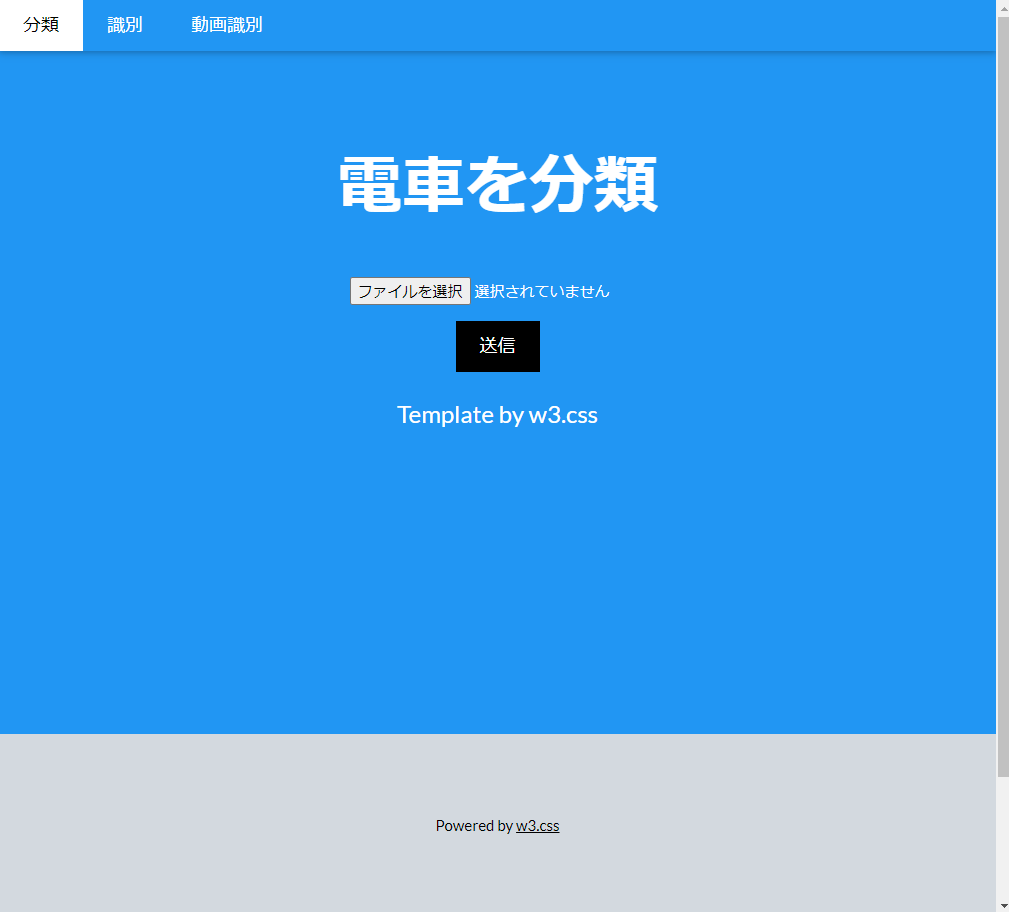
\includegraphics [width=\linewidth]{chap2/fig/pc_index.png}%配置するチャプターに応じて変えて
			\caption{PCで見た際のindex.html}	\label{fig_pc_index}
		\end{minipage}	
		\begin{minipage}[b]{0.45\textwidth}
			\centering
			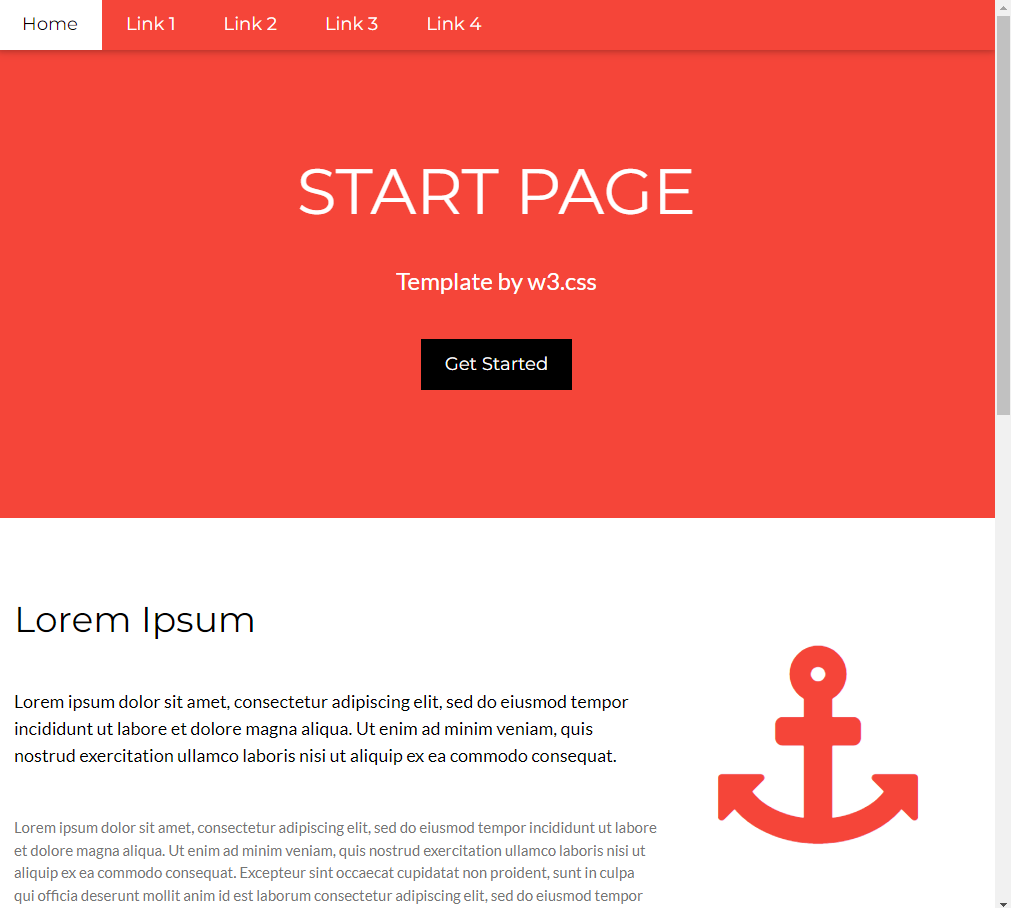
\includegraphics [width=\linewidth]{chap2/fig/pc_template.png}%配置するチャプターに応じて変えて
			\caption{テンプレートの見た目}\label{fig_pc_template}
		\end{minipage}
	\end{tabular}
\end{figure}



\section{動作確認と現状}
\subsection{電車の画像の分類} 
出力後の画面を図\ref{img_cls}に示す.
この機能では,ユーザがブラウザからアップロードした画像に含まれる電車の種類を分類する. 分類の結果,最も可能性が高いものをWebページに出力する.
\subsection{電車の画像の識別}
出力後の画面を図\ref{img_det}に示す.
この機能では,ユーザがブラウザからアップロードした画像に含まれる電車の位置と種類を識別する.  識別の結果,バウンディングボックスが追加された画像をWebページに表示する.
\subsection{電車の動画の識別} 
出力後の画面を図\ref{mov_det}に示す.
この機能では,ユーザがブラウザからアップロードした動画に含まれる電車の位置と種類を識別する. 識別の結果,バウンディングボックスが追加された動画をWebページに表示する.

%\begin{figure}
%	\centering
%	\includegraphics[width=0.5\linewidth]{obj/image1.png}
%	\figcap{画像の分類}{classify image}{cls-img}
%\end{figure}

\begin{figure}[H]
	\begin{tabular}{ccc}
		\begin{minipage}[b]{0.3\textwidth}
			\centering
			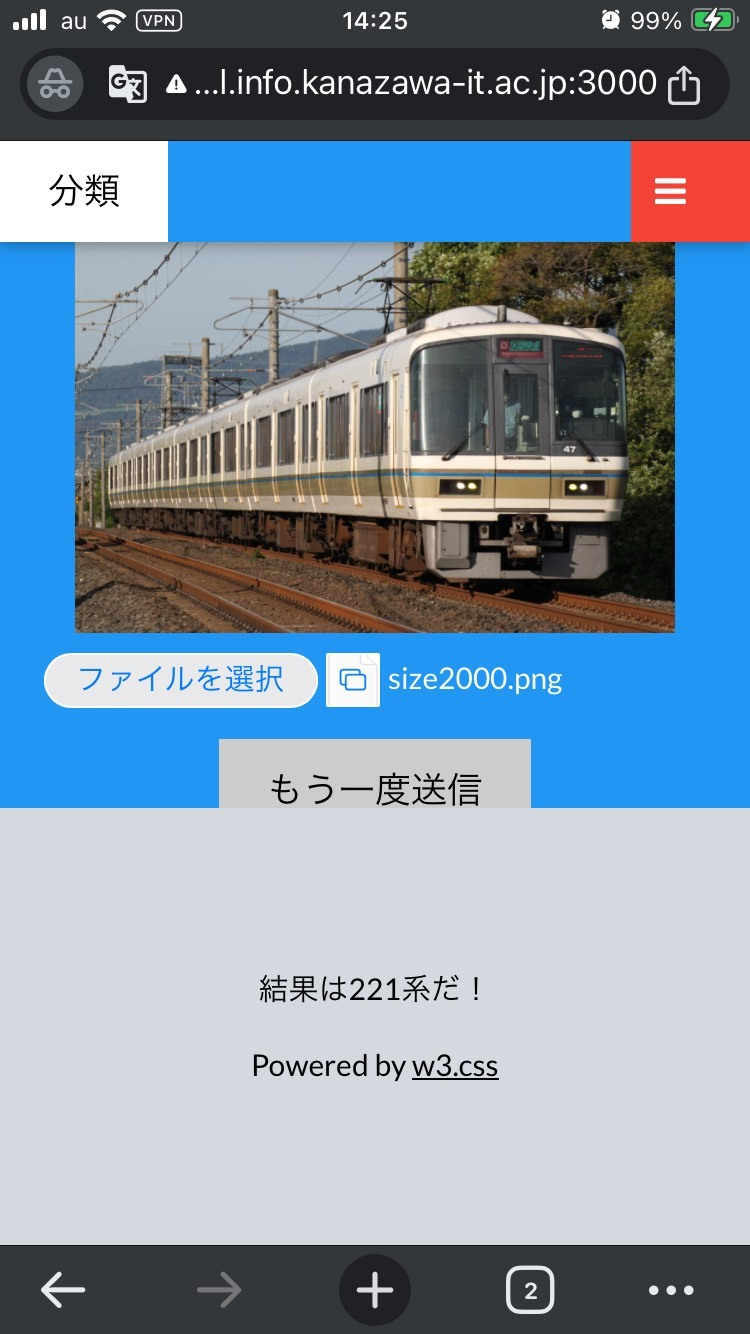
\includegraphics[width=\linewidth]{chap2/fig/img_classify.jpg}
			\caption{画像の分類}
			\label{img_cls}
		\end{minipage}
		\begin{minipage}[b]{0.3\textwidth}
			\centering
			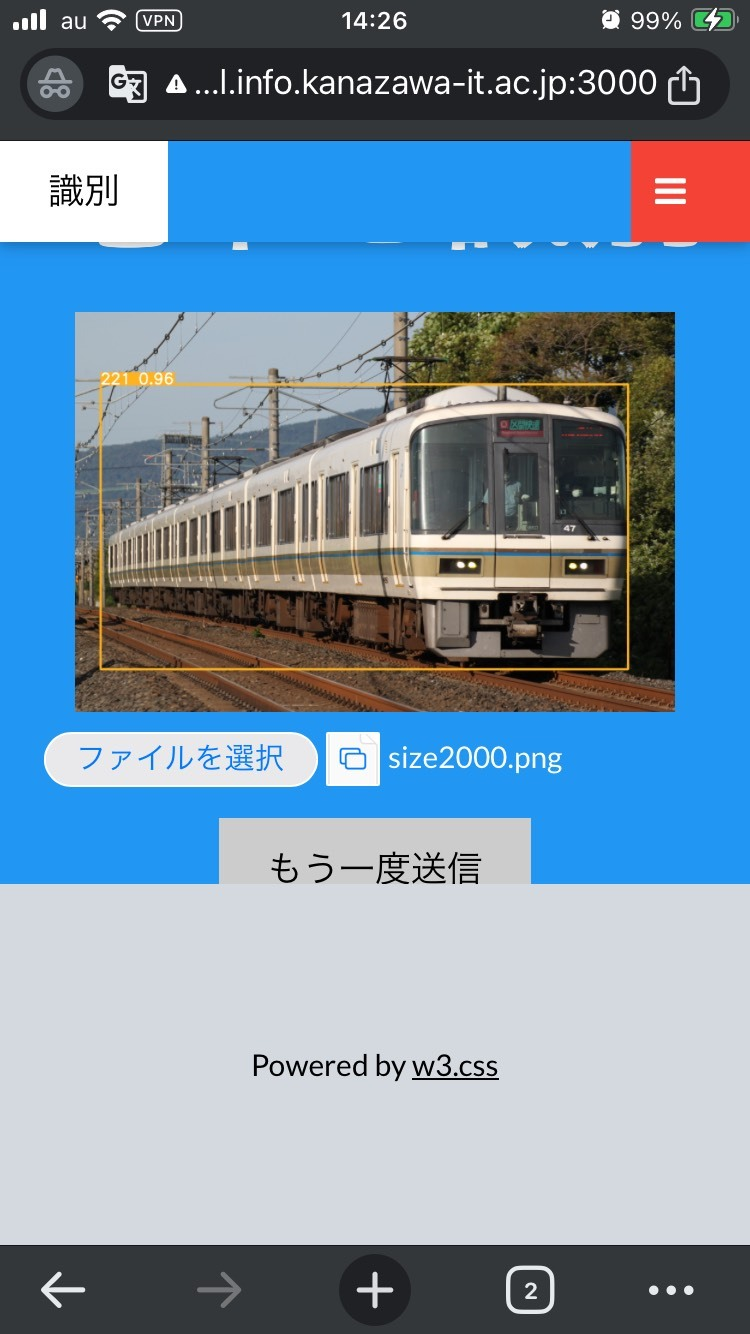
\includegraphics[width=\linewidth]{chap2/fig/img_identify.jpg}
			\caption{画像の識別}
			\label{img_det}
		\end{minipage}
		\begin{minipage}[b]{0.3\textwidth}
			\centering
			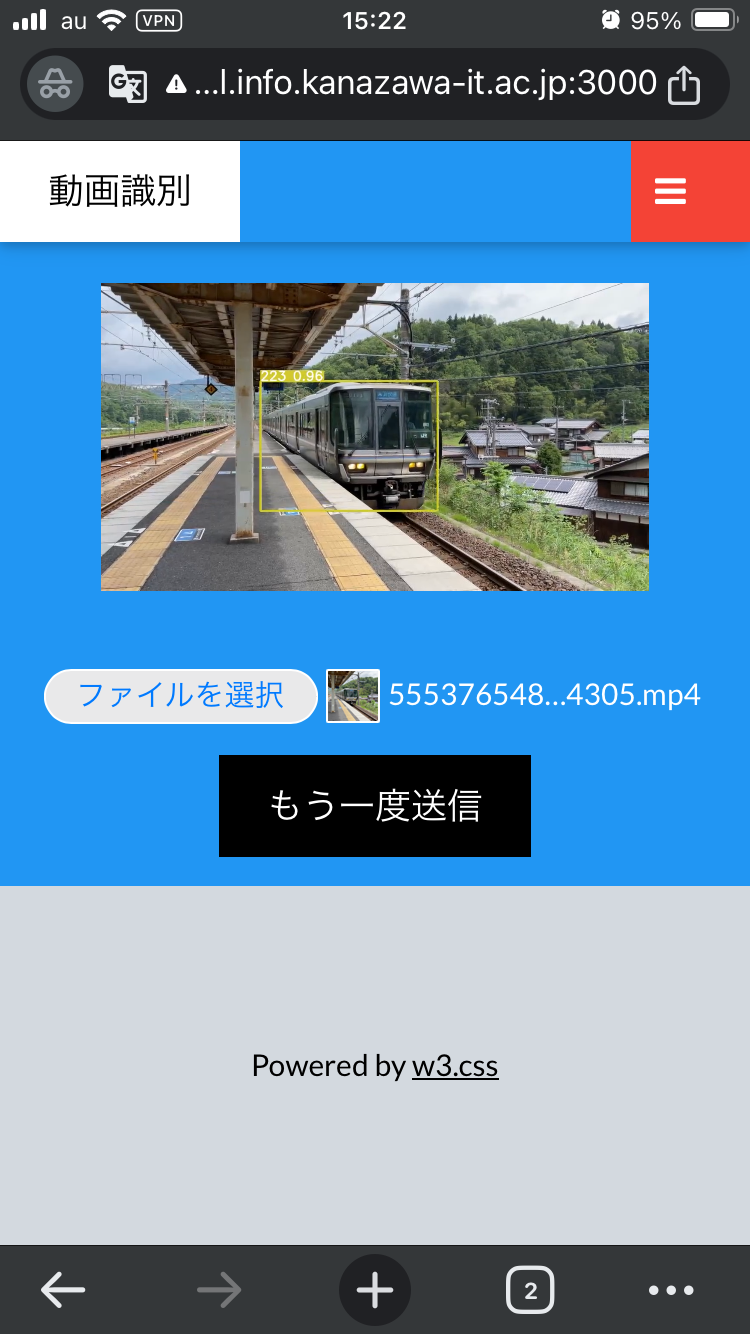
\includegraphics[width=\linewidth]{chap2/fig/mov_identify1.jpg}
			\caption{動画の識別}
			\label{mov_det}
		\end{minipage}
	\end{tabular}
\end{figure}
